\documentclass[12pt]{article}
\usepackage{amsmath}
\usepackage{graphicx}
\usepackage{hyperref}
\usepackage{listings}
\usepackage{color}
\usepackage{pythonhighlight}
\usepackage{enumerate} 

\title{Operating System Course Report - First Half of the Semester}
\author{A class}
\date{\today}

\begin{document}

\maketitle
\newpage

\tableofcontents
\newpage

\section{Introduction}
This report summarizes the topics covered during the first half of the Operating System course. It includes theoretical concepts, practical implementations, and assignments. The course focuses on the fundamentals of operating systems, including system architecture, process management, CPU scheduling, and deadlock handling.

\section{Course Overview}
\subsection{Objectives}
The main objectives of this course are:
\begin{itemize}
    \item To understand the basic components and architecture of a computer system.
    \item To learn process management, scheduling, and inter-process communication.
    \item To explore file systems, input/output management, and virtualization.
    \item To study the prevention and handling of deadlocks in operating systems.
\end{itemize}

\subsection{Course Structure}
The course is divided into two halves. This report focuses on the first half, which covers:
\begin{itemize}
    \item Basic Concepts and Components of Computer Systems
    \item System Performance and Metrics
    \item System Architecture of Computer Systems
    \item Process Description and Control
    \item Scheduling Algorithms
    \item Process Creation and Termination
    \item Introduction to Threads
    \item File Systems
    \item Input and Output Management
    \item Deadlock Introduction and Prevention
    \item User Interface Management
    \item Virtualization in Operating Systems
\end{itemize}

\section{Topics Covered}

\subsection{Basic Concepts and Components of Computer Systems}
 \hspace{0.61cm}Secara harfiah Sistem dalam bahasa Latin : \textit{systema} Yunani : \textit{sustema}, suatu kesatuan yang berhubungan. Komputer adalah alat elektronik yang digunakan untuk mengolah data. Sistem komputer secara umum adalah sebuah kesatuan dari berbagai komponen yang bekerja bersama untuk mengolah data dan informasi. 

\subsubsection{ Jenis-Jenis Komputer } 

\begin{enumerate}
    \item \textbf{\textit{Personal Computer} (PC)}
    
    \hspace{0.61cm}\textit{Personal Computer} (PC) atau komputer pribadi adalah jenis komputer yang paling sering digunakan oleh banyak orang untuk kebutuhan pribadi sehari-hari. Anda biasa melihat jenis komputer ini di kantor, rumah, toko, atau tempat lainnya yang penggunaannya hanya untuk memenuhi kebutuhan perorangan saja. 

    \hspace{0.61cm}\textit{Personal Computer} memiliki ukuran yang kecil sehingga membuatnya nyaman untuk digunakan. Selain itu, biaya produksinya rendah dan harganya juga murah. Dengan kecepatan komputasi yang mencapai ratusan hingga jutaan ribu instruksi per jam, membuat PC sudah memenuhi persyaratan untuk memproses data dan komputasi ilmiah dalam hal produksi, penelitian ilmiah, serta kehidupan sehari-hari. 

    \hspace{0.61cm}Sebenarnya, fungsi utama jenis komputer ini adalah untuk mengelola data \textit{input output} sederhana. Namun, sudah banyak orang yang menggunakannya untuk bermain \textit{games}, membuka web, mengerjakan dokumen, bahkan digunakan sebagai mesin kasir toko. 
    
    \item \textbf{Komputer Desktop}

    \hspace{0.61cm}Jenis komputer yang kedua yaitu komputer desktop. Jenis komputer ini dirancang khusus untuk memenuhi kebutuhan rumah dan kantor. Sebagai contoh untuk menyelesaikan pekerjaan atau pengelolaan data kantoran. Pada umumnya, komputer ini hadir dengan jenis \textit{keyboard, monitor,} dan CPU yang dirancang secara terpisah dengan ukuran yang besar. 
    
    \item \textbf{Laptop}
    
    \hspace{0.61cm}Laptop adalah salah satu jenis komputer desktop yang berevolusi sehingga memiliki ukuran yang lebih kecil, mulai dari \textit{monitor}, CPU, hingga \textit{keyboard}. Hal menarik dari laptop adalah komponennya yang terangkum menjadi satu perangkat saja sehingga mudah untuk dibawah kemana pun oleh penggunanya. Penyimpanannya jadi lebih mudah karena bentuknya yang ringkas. 

    \hspace{0.61cm}Sudah ada banyak jenis laptop yang dijual dengan berbagai macam spesifikasi, mulai dari yang rendah hingga tinggi. Anda bisa melihatnya dari kapasitas RAM, ROM, dan \textit{harddisk} yang digunakan. Oleh sebab itu, Anda bisa memilih laptop sesuai dengan kebutuhan sehari-hari.

    \item \textbf{Komputer Tablet} 

    \hspace{0.61cm}Komputer tablet merupakan perangkat komputer\textit{ portabel} yang memiliki layar sentuh dan dirancang untuk mobilitas dan produktivitas pengguna. Sama halnya dengan laptop, komputer tablet juga memiliki komponen yang terangkum menjadi satu perangkat saja agar memudahkan untuk dibawa kemanapun oleh pengguna. 

    \hspace{0.61cm}Dengan komputer tablet, Anda bisa melakukan berbagai macam aktivitas seperti membaca buku, menjelajah web, menonton film, mendengarkan musik, hingga bermain \textit{games} di mana pun dan kapan pun. Selain itu, komputer tablet juga memiliki daya tahan baterai yang lebih lama dan mesin grafis terintegrasi sehingga Anda bisa menggunakannya lebih lama dan nyaman karena memiliki visual yang lebih baik. 

    \item \textbf{Komputer \textit{Server}} 

    \hspace{0.61cm}Komputer \textit{server} merupakan jenis komputer yang dirancang khusus untuk memberikan data, layanan, atau sumber daya untuk komputer lain dalam jaringan. Komputer ini dilengkapi dengan prosesor yang sangat kuat serta bisa menampung daya besar mulai dari \textit{hard-disk}, RAM, dan perangkat lainnya. 

    \hspace{0.61cm}Biasanya, jenis komputer ini bekerja secara terus menerus karena memang dirancang untuk kinerja dan keandalan yang tinggi. Komputer \textit{server} sendiri terdiri dari beberapa macam jenis, yaitu \textit{server file, server web, server database,} dan \textit{server FTP}. 

    \item \textbf{Komputer \textit{Hybrid} }
    
    \hspace{0.61cm}Komputer \textit{hybrid} merupakan jenis komputer yang dirancang khusus agar dapat bekerja secara kuantitatif atau kualitatif. Umumnya, komputer ini digunakan untuk menggerakkan mesin atau robot. Anda akan menemukan jenis komputer ini di pabrik-pabrik yang memproduksi barang dengan bantuan mesin.

    \item \textbf{Komputer \textit{Workstation}}

    \hspace{0.61cm}Komputer \textit{workstation} merupakan jenis komputer yang memiliki kapasitas memori, penyimpanan eksternal, serta tampilan layar yang besar. Komputer ini juga hadir dengan kemampuan memproses data dan memproses grafik yang kuat. Umumnya, komputer \textit{workstation} dirancang dan dikembangkan untuk aplikasi profesional karena memiliki kinerja serta kemampuan grafis yang tinggi. 

    \hspace{0.61cm}Maka dari itu, jenis komputer ini banyak digunakan untuk keperluan animasi 3D, desain grafis, pengembangan perangkat lunak, layanan informasi, dan berbagai bidang lainnya yang membutuhkan penggunaan program berat. 

    \item \textbf{Komputer \textit{Mainframe}}

    \hspace{0.61cm}Komputer \textit{mainframe} merupakan jenis komputer besar yang dapat menangani serta memproses data dalam jumlah yang besar dengan cepat. Komputer ini memiliki kecepatan kalkulasi hingga mencapai jutaan hingga puluhan juta pengguna sekaligus. Jenis komputer ini juga terkenal karena kemampuannya untuk mengelola banyak tugas sekaligus. 

    \hspace{0.61cm}Biasanya, komputer ini digunakan di organisasi atau institusi besar seperti bank, pemerintahan, atau perusahaan besar yang sering memproses volume data yang sangat besar. Itu dia penjelasan mengenai jenis-jenis komputer. Dengan mengetahui jenis dan fungsinya, Anda jadi bisa memilih jenis komputer mana yang cocok digunakan untuk kebutuhan sehari-hari.
    
\end{enumerate}

\subsection{System Performance and Metrics}
This section introduces various system performance metrics used to measure the efficiency of a computer system, including throughput, response time, and utilization.

\subsection{System Architecture of Computer Systems}
Describes the architecture of modern computer systems, focusing on the interaction between hardware and the operating system.

\subsection{Process Description and Control}
Processes are a central concept in operating systems. This section covers:
\begin{itemize}
    \item Process states and state transitions
    \item Process control block (PCB)
    \item Context switching
\end{itemize}

\subsection{Scheduling Algorithms}
This section covers:
\begin{itemize}
    \item First-Come, First-Served (FCFS)
    \item Shortest Job Next (SJN)
    \item Round Robin (RR)
\end{itemize}
It explains how these algorithms are used to allocate CPU time to processes.

\subsection{Process Creation and Termination}
Details how processes are created and terminated by the operating system, including:
\begin{itemize}
    \item Process spawning
    \item Process termination conditions
\end{itemize}

\subsection{Introduction to Threads}
This section introduces the concept of threads and their relation to processes, covering:
\begin{itemize}
    \item Single-threaded vs. multi-threaded processes
    \item Benefits of multithreading
\end{itemize}

\begin{figure}[h]
    \centering
    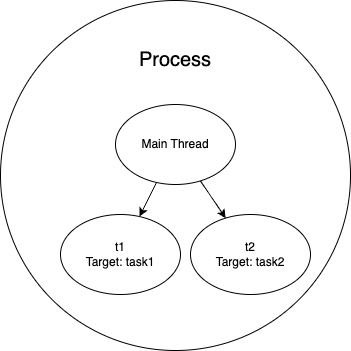
\includegraphics[width=0.5\textwidth]{/Users/khawaritzmi/Unhas/os_report_mid2024/b_class/asset/example.png}  % Sesuaikan nama file dan ukurannya
    \caption{Ini adalah gambar contoh dari multithreading.}
    \label{fig:contoh_gambar}
\end{figure}

Seperti yang terlihat pada Gambar \ref{fig:contoh_gambar}, inilah cara menambahkan gambar dengan keterangan.

\subsection{File Systems}
File systems provide a way for the operating system to store, retrieve, and manage data. This section explains:
\begin{itemize}
    \item File system structure
    \item File access methods
    \item Directory management
\end{itemize}

\subsection{Input and Output Management}
Input and output management is key for handling the interaction between the system and external devices. This section includes:
\begin{itemize}
    \item Device drivers
    \item I/O scheduling
\end{itemize}

\subsection{Deadlock Introduction and Prevention}
Explores the concept of deadlocks and methods for preventing them:
\begin{itemize}
    \item Deadlock conditions
    \item Deadlock prevention techniques
\end{itemize}

\subsection{User Interface Management}
This section discusses the role of the operating system in managing the user interface. Topics covered include:
\begin{itemize}
    \item Graphical User Interface (GUI)
    \item Command-Line Interface (CLI)
    \item Interaction between the user and the operating system
\end{itemize}

\subsection{Virtualization in Operating Systems}
Virtualization allows multiple operating systems to run concurrently on a single physical machine. This section explores:
\begin{itemize}
    \item Concept of virtualization
    \item Hypervisors and their types
    \item Benefits of virtualization in modern computing
\end{itemize}

\section{Assignments and Practical Work}
\subsection{Assignment 1: Process Scheduling}
Students were tasked with implementing various process scheduling algorithms (e.g., FCFS, SJN, and RR) and comparing their performance under different conditions.
\subsubsection{Group 1}
\begin{python}
    class Process:
    def __init__(self, pid, arrival_time, burst_time):
        self.pid = pid
        self.arrival_time = arrival_time
        self.burst_time = burst_time
        self.completion_time = 0
        self.turnaround_time = 0
        self.waiting_time = 0
\end{python}

\begin{table}[htbp] % Optional: For floating position
    \centering
    \begin{tabular}{|c|c|c|} % Defines number of columns and alignment (c = center, l = left, r = right). '|' creates vertical lines.
    \hline
    Header 1 & Header 2 & Header 3 \\ % Column headers
    \hline
    Row 1, Column 1 & Row 1, Column 2 & Row 1, Column 3 \\ % First row of data
    \hline
    Row 2, Column 1 & Row 2, Column 2 & Row 2, Column 3 \\ % Second row of data
    \hline
    \end{tabular}
    \caption{Your table caption} % Optional: For adding a caption
    \label{tab:your_label} % Optional: For cross-referencing the table
\end{table}

\subsection{Assignment 2: Deadlock Handling}
In this assignment, students were asked to simulate different deadlock scenarios and explore various prevention methods.

\subsubsection{Group 1}
\subsection*{Soal}

\begin{enumerate}
    \item Simulasikan beberapa skenario \textit{deadlock} dengan menggunakan pemrograman \textit{Python}. Skenario-skenario tersebut harus mencakup situasi di mana dua atau lebih proses saling menunggu satu sama lain untuk melepaskan sumber daya.

    \item Eksplorasi beberapa metode pencegahan \textit{deadlock} berikut ini:
    \begin{itemize}
        \item  {Prevention}: Buat aturan sehingga deadlock tidak mungkin terjadi.
        \item {Avoidance}: Simulasikan algoritma \textit{Banker's} untuk menghindari \textit{deadlock}.
        \item {Detection and Recovery}: Implementasikan mekanisme untuk men-deteksi \textit{deadlock} dan mengambil langkah pemulihan.
    \end{itemize}
    Setiap metode, tunjukkan bagaimana cara metode tersebut bekerja melalui implementasi \textit{Python.} Serta berikan analisis singkat dari setiap pendekatan, termasuk kelebihan dan kekurangannya.
\end{enumerate}

\subsection*{Jawaban}

\begin{enumerate}
    \item Skenario \textit{Deadlock}

    Pada skenario ini, kita akan membuat dua atau lebih proses yang membutuhkan dua sumber daya dan mengunci satu sama lain, menciptakan situasi \textit{deadlock}.


    Kode \textit{Phyton}:

    \begin{python}
import threading
import time

lock1 = threading.Lock()
lock2 = threading.Lock()

def process_1():
    print("Process 1 trying to lock resource 1")
    lock1.acquire()
    print("Process 1 locked resource 1")
    time.sleep(1)
    
    print("Process 1 trying to lock resource 2")
    lock2.acquire()
    print("Process 1 locked resource 2")
    
    lock2.release()
    lock1.release()

def process_2():
    print("Process 2 trying to lock resource 2")
    lock2.acquire()
    print("Process 2 locked resource 2")
    time.sleep(1)
    
    print("Process 2 trying to lock resource 1")
    lock1.acquire()
    print("Process 2 locked resource 1")
    
    lock1.release()
    lock2.release()

t1 = threading.Thread(target=process_1)
t2 = threading.Thread(target=process_2)

t1.start()
t2.start()

t1.join()
t2.join()

    \end{python}

    Hasil : Pada simulasi ini, proses pertama mengunci \textit{resource} 1 lalu mencoba mengunci \textit{resource} 2, sementara proses kedua mengunci \textit{resource} 2 dan mencoba mengunci \textit{resource} 1, sehingga kedua proses saling menunggu dan terjadi \textit{deadlock.}

    \item Skenario Pencegahan \textit{Deadlock}

    Untuk mencegah \textit{deadlock} kita bisa menggunakan metode - metode berikut:

    \begin{enumerate}[a.]
        \item \textit{Prevention} (Pencegahan \textit{Deadlock})

        Dalam metode pencegahan, kita mencegah \textit{deadlock} dengan me-netapkan aturan tertentu, seperti memaksa semua proses untuk mengunci \textit{resource} dalam urutan yang sama.
    \end{enumerate}

    Kode\textit{Phyton} :

    \begin{python}
def process_1_prevention():
    print("Process 1 trying to lock resources in order")
    lock1.acquire()
    print("Process 1 locked resource 1")
    time.sleep(1)
    
    lock2.acquire()
    print("Process 1 locked resource 2")
    
    lock2.release()
    lock1.release()
def process_2_prevention():
    print("Process 2 trying to lock resources in order")
    lock1.acquire()
    print("Process 2 locked resource 1")
    time.sleep(1)
    
    lock2.acquire()
    print("Process 2 locked resource 2")
    
    lock2.release()
    lock1.release()

t1 = threading.Thread(target=process_1_prevention)
t2 = threading.Thread(target=process_2_prevention)

t1.start()
t2.start()

t1.join()
t2.join()
    \end{python}

    Analisis : Metode pencegahan ini memastikan bahwa semua proses mengunci \textit{resource} dalam urutan yang sama sehingga \textit{deadlock} tidak akan terjadi. Namun, metode ini bisa mengurangi fleksibilitas dan efisiensi dalam penggunaan \textit{resource.}

    \begin{enumerate}[b.]
        \item {Avoidance} (Algoritma \textit{Banker's})

        Metode ini menggunakan algoritma \textit{Banker's} yang menghitung apa-kah permintaan sumber daya dapat dipenuhi tanpa menyebabkan \textit{deadlock}. Berikut adalah contoh sederhana simulasi \textit{Banker's algorithm.}
    \end{enumerate}

        Kode \textit{Phyton} :

        \begin{python}
def is_safe(available, max_need, allocation):
    need = [[max_need[i][j] - allocation[i][j] for j in range(len(available))] for i in range(len(allocation))]
    work = available[:]
    finish = [False] * len(allocation)
    safe_sequence = []

while len(safe_sequence) < len(finish):
    for i in range(len(finish)):
        if not finish[i] and all(need[i][j] <= work[j] for j in range(len(work))):
            safe_sequence.append(i)
            work = [work[j] + allocation[i][j] for j in range(len(work))]
            finish[i] = True
            break
    else:
        return False, []

return True, safe_sequence

available = [3, 3, 2]
max_need = [[7, 5, 3], [3, 2, 2], [9, 0, 2], [2, 2, 2], [4, 3, 3]]
allocation = [[0, 1, 0], [2, 0, 0], [3, 0, 2], [2, 1, 1], [0, 0, 2]]

is_safe_state, safe_seq = is_safe(available, max_need, allocation)
if is_safe_state:
    print(f"System is in safe state. Safe sequence: {safe_seq}")
else:
    print("System is in unsafe state. Deadlock may occur.")
    \end{python}

    Analisis : Algoritma \textit{Banker's} menjaga sistem tetap dalam keadaan aman. Kelebihannya adalah algoritma ini memastikan bahwa \textit{deadlock} tidak akan terjadi. Namun, kerugiannya adalah algoritma ini memerlukan informasi yang akurat tentang jumlah sumber daya yang dibutuhkan setiap proses dan sering kali terlalu konservatif.

    \begin{enumerate}[c.]
        \item \textit{Detection and Recovery} (Pendeteksian dan Pemulihan \textit{Deadlock)}

        Metode ini mendeteksi \textit{deadlock} dengan memonitor kondisi sistem, kemudian mengambil tindakan pemulihan seperti menghentikan beberapa proses untuk memecah \textit{deadlock}.
    \end{enumerate}

    Kode \textit{python}:

    \begin{python}
def detect_deadlock(allocation, request, available):
    num_processes = len(allocation)
    num_resources = len(available)

    finish = [False] * num_processes
    work = available[:]

    while True:
        found_process = False
        for i in range(num_processes):
            if not finish[i] and all(request[i][j] <= work[j] for j in range(num_resources)):
                for j in range(num_resources):
                    work[j] += allocation[i][j]
                finish[i] = True
                found_process = True
        if not found_process:
            break

    if all(finish):
        return False
    else:
        return True

allocation = [[0, 1, 0], [2, 0, 0], [3, 0, 2], [2, 1, 1], [0, 0, 2]]
request = [[0, 0, 0], [2, 0, 2], [0, 0, 0], [1, 0, 0], [0, 0, 2]]
available = [0, 0, 0]

if detect_deadlock(allocation, request, available):
    print("Deadlock detected.")
else:
    print("No deadlock.")
    \end{python}

    Analisis : Metode deteksi dan pemulihan efektif dalam situasi di mana \textit{deadlock} jarang terjadi. Keuntungannya adalah sumber daya dapat digunakan lebih optimal tanpa harus mencegah \textit{deadlock} sejak awal. Namun, pemulihan bisa memerlukan penghentian proses, yang mungkin tidak selalu diinginkan.
\end{enumerate}

\subsection{Assignment 3: Multithreading and Amdahl's Law}
This assignment involved designing a multithreading scenario to solve a computationally intensive problem. Students then applied **Amdahl's Law** to calculate the theoretical speedup of the program as the number of threads increased.

\subsection{Assignment 4: Simple Command-Line Interface (CLI) for User Interface Management}
Students were tasked with creating a simple **CLI** for user interface management. The CLI should support basic commands such as file manipulation (creating, listing, and deleting files), process management, and system status reporting.

\subsection{Assignment 5: File System Access}
In this assignment, students implemented file system access routines, including:
\begin{itemize}
    \item File creation and deletion
    \item Reading from and writing to files
    \item Navigating directories and managing file permissions
\end{itemize}

\section{Conclusion}
The first half of the course introduced core operating system concepts, including process management, scheduling, multithreading, and file system access. These topics provided a foundation for more advanced topics to be covered in the second half of the course.

\end{document}